\documentclass{article}
\usepackage[utf8]{inputenc}
\usepackage[fleqn]{amsmath}
\usepackage{gensymb}
\usepackage{amssymb}
\usepackage{mathtools}
\usepackage{array}
\usepackage[T1]{fontenc}
\usepackage[margin=1in]{geometry}
\usepackage{tabularx}
\usepackage{pesmath}
\usepackage{fancyhdr}
\usepackage{graphicx}
\usepackage[russian]{babel}
\usepackage{mathrsfs}
\usepackage[verbose]{placeins}
\graphicspath{{images/}}
 
\title{\textbf{Оптимизация при помощи LLM}}
\date{}
\pagestyle{fancy}
\fancyhf{}
\rhead{Инновационный практикум}
\chead{Тезисы}
\rfoot{\thepage}


\begin{document}
\maketitle
\begin{flushleft}
\paragraph{}
В работе рассматривается архитектура Discrete Neural Algorithmic Reasoning \cite{rodionov2025discreteneuralalgorithmicreasoning} в контексте алгоритмических задач дискретной оптимизации. 
\paragraph{}
Данная архитектура воспроизводит пошаговое выполнение алгоритмов на графах помощью механизмов hard graph attention \cite{rodionov2025discreteneuralalgorithmicreasoning}. С учётом того, что любое представление входных данных может быть сведено к графовому виду, модель легко применяется к любой алгоритмической задаче. 
\paragraph{}
Преимущество модели по отношению к обычным методам состоит в том, что архитектура не чувствительна к размерности задачи, что даёт возможность проводить обучение на задачах меньшей размерности и проводить inference за полиномиальное время в силу устройства архитектуры.

\paragraph{}
Коротко о метриках, используемых нами и непосредственно авторами архитектуры. Для каждого шага алгоритма в зависимости от типа состояний задачи выбирается метрика, которая оценивает правильность предсказаний на уровне одной вершины/ребра (например pointer accuracy). Метрика на графовом уровне равна 1, если все локальные метрики равны 1, иначе -- 0. Обе метрики усредняются по всему датасету задач-графов.
\section*{1. Графовые задачи}
\paragraph{}{В процессе исследования рассмотрено применение архитектуры к задаче поиска кратчайшего пути, а именно посредством воспроизведения алгоритма Дийкстры. Итоговые метрики: pointer\_accuracy = 1, pointer\_accuracy\_graph\_level = 1.}
\paragraph{}
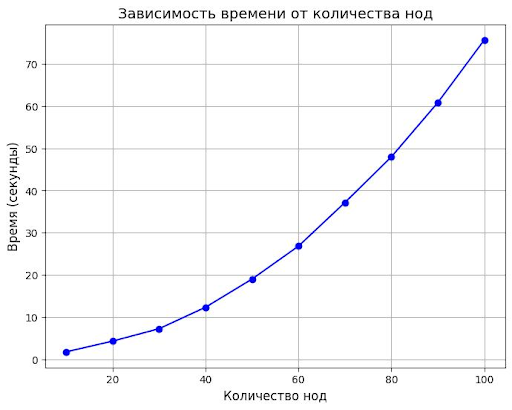
\includegraphics[width=0.5\linewidth]{dijkstra.png}
\section*{2. Неграфовые задачи}
\paragraph{}
Также рассмотрено применение к неграфовым задачам на примере задачи SAT. Мы использовали сведение этой задачи к задаче поиска максимального независимого множества. Эту задачу мы решали рандомизированным алгоритмом Луби \cite{ghaffari2015improveddistributedalgorithmmaximal}. Архитектура успешно обучается, доля правильно решенных формул высокая при оптимальном фиксированном ограничении сверху на число шагов алгоритма (рассматривалось одинаковое ограничение для всех вариантов формул).
\paragraph{}
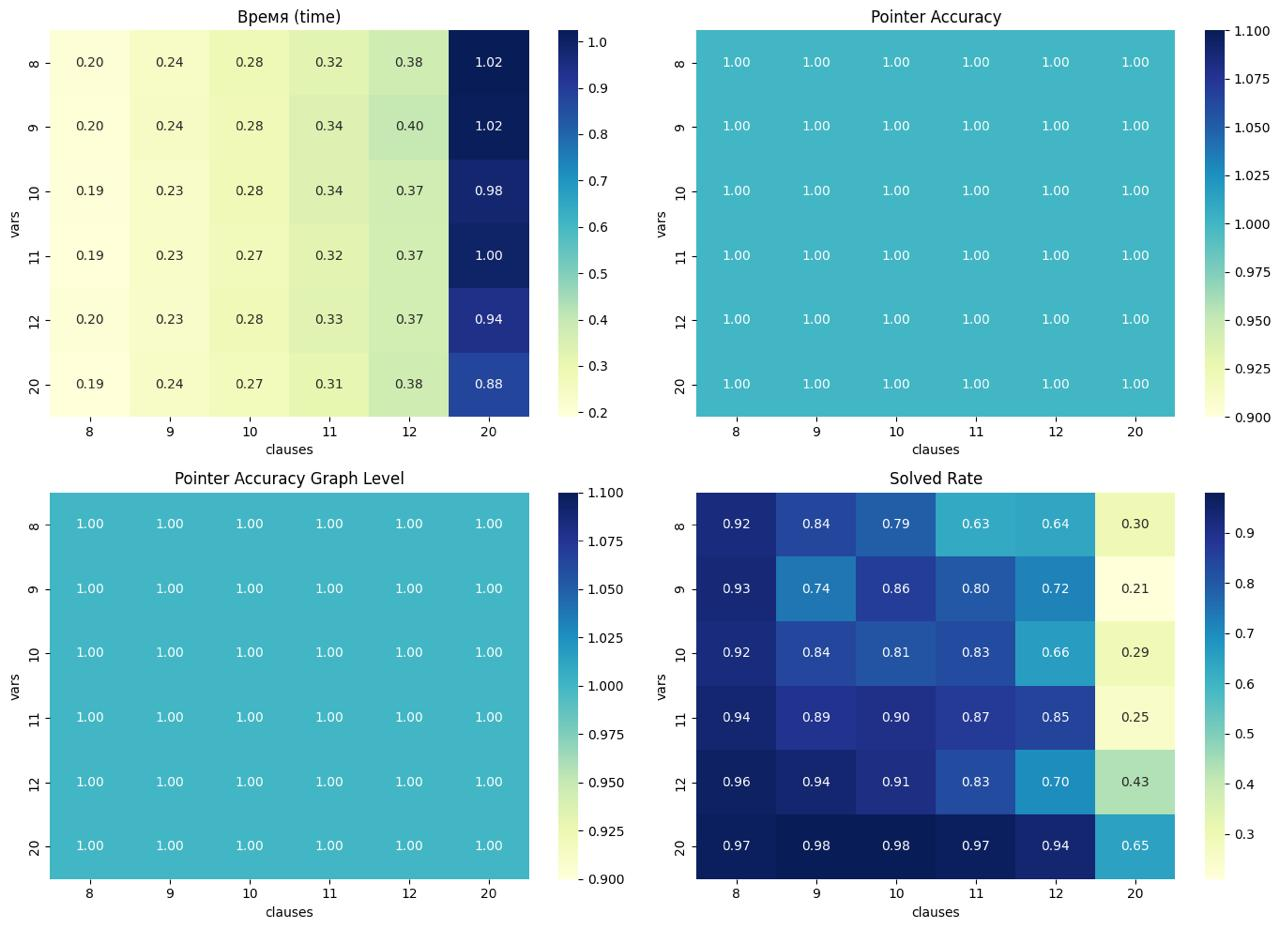
\includegraphics[width=0.7\linewidth]{sat.png}
\section*{3. Оптимизация по времени}
В контексте задач дискретной оптимизации важно оптимизировать время работы. Поэтому мы реализовали версию архитектуры, в котором квадратичный Attention был заменен линейной Mamba \cite{gu2024mambalineartimesequencemodeling}.
На текущей момент рассмотрены задачи малой размерности (задача кратчайшего пути с алгоритмом Дийкстры). Архитектура обучается, но значимого выигрыша по времени на таких размерностях не наблюдается. В процессе исследования -- инференс на задачах большой размерности.
\paragraph{}
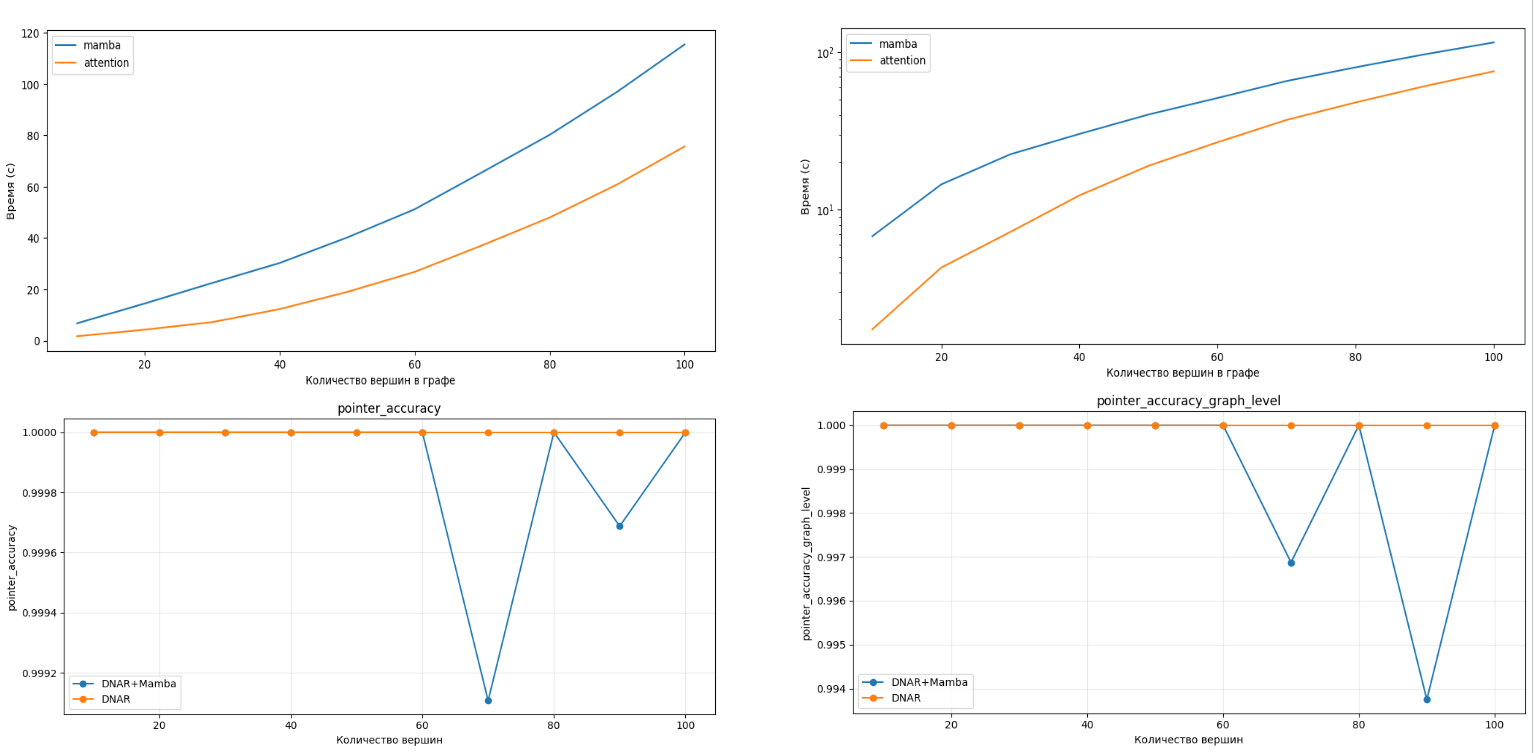
\includegraphics[width=0.7\linewidth]{mamba.png}
\section*{4. Mixed integer linear programming problem}
\paragraph{}
Рассмотрено применение к задаче MILP. Была рассмотрена версия алгоритма Branch\&Bound \cite{huang2021branchboundmixedinteger} с одновременным использованием стратегий Depth-first search и ветвления по `наиболее дробной` переменной. Без добавления шагов LP-солвера (релаксация к которому является частью этого алгоритма) в обучающий датасет, архитектура не продемонстрировала способность к обучению.
\paragraph{}
Удалось применить архитектуру для выбора переменной ветвления в комбинации с внешним lp-солвером в роли оракула. Преимуществ по сравнению с обычным подходом такая комбинация не представляет (сравнение по времени на случайных задачах показано на графике). Однако остаётся возможность для обобщения архитектурой большого множества известных эвристик для Branch\&Bound (например применение наиболее оптимальной эвристики в зависимости от задачи) -- данная часть в процессе исследования.
\paragraph{}

\includegraphics[width=0.7\linewidth]{milp.png}
\bibliographystyle{plain}
\bibliography{references}
\end{flushleft}
\end{document}
